\chapter{The History and Downfall of Money}
\label{les:12}

\begin{chapquote}{Lewis Carroll, \textit{Alice in Wonderland}}
``They would not remember the simple rules their friends had given them, such
as, that, if you get into the fire, it will burn you, and that, if you cut your
finger very deeply with a knife, it generally bleeds, and she had never
forgotten that, if you drink a bottle marked `poison,' it is almost certain to
disagree with you, sooner or later.''
\end{chapquote}

Many people think that money is backed by gold, which is locked away in
big vaults, protected by thick
walls. This ceased to be true many decades ago. I am not sure what I
thought, since I was in much deeper trouble, having virtually no
understanding of gold, paper money, or why it would need to be backed by
something in the first place.

One part of learning about Bitcoin is learning about fiat money: what it
means, how it came to be, and why it might not be the best idea we ever
had. So, what exactly is fiat money? And how did we end up using it?

If something is imposed by \textit{fiat}, it simply means that it is imposed by
formal authorization or proposition. Thus, fiat money is money simply
because \textit{someone} says that it is money. Since all governments use fiat
currency today, this someone is \textit{your} government. Unfortunately, you
are not \textit{free} to disagree with this value proposition. You will quickly
feel that this proposition is everything but non-violent. If you refuse
to use this paper currency to do business and pay taxes the only people
you will be able to discuss economics with will be your cellmates.

The value of fiat money does not stem from its inherent properties. How
good a certain type of fiat money is, is only correlated to the
political and fiscal (in)stability of those who dream it into existence.
Its value is imposed by decree, arbitrarily.

\begin{figure}
  \centering
  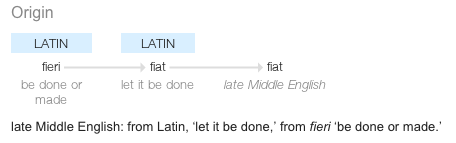
\includegraphics[width=8cm]{assets/images/fiat-definition.png}
  \caption{fiat --- 'Let it be done'}
  \label{fig:fiat-definition}
\end{figure}

Until recently, two types of money were used: \textbf{commodity money}, made
out of precious \textit{things}, and \textbf{representative money}, which simply
\textit{represents} the precious thing, mostly in writing.

We already touched on commodity money above. People used special bones,
seashells, and precious metals as money. Later on, mainly coins made out of
precious metals like gold and silver were used as money. The oldest coin found
so far is made of a natural gold-and-silver mix and was made more than 2700
years ago.\footnote{According to the Greek historian Herodotus, writing in the
fifth century BC, the Lydians were the first people to have used gold and silver
coinage. \cite{coinage-origins}} If something is new in Bitcoin, the concept of
a coin is not it.

\begin{figure}
  \centering
  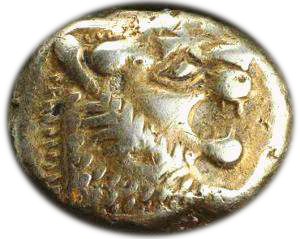
\includegraphics[width=5cm]{assets/images/lydian-coin-stater.png}
  \caption{Lydian electrum coin}
  \label{fig:lydian-coin-stater}
\end{figure}

Turns out that hoarding coins, or hodling, to use today's parlance, is
almost as old as coins. The earliest coin hodler was someone who put
almost a hundred of these coins in a pot and buried it in the
foundations of a temple, only to be found 2500 years later. Pretty good
cold storage if you ask me.

One of the downsides of using precious metal coins is that they can be
clipped, effectively debasing the value of the coin. New coins can be
minted from the clippings, inflating the money supply over time,
devaluing every individual coin in the process. People were literally
shaving off as much as they could get away with of their silver dollars.
I wonder what kind of \textit{Dollar Shave Club} advertisements they had back
in the day.

Since governments are only cool with inflation if they are the ones
doing it, efforts were made to stop this guerrilla debasement. In
classic cops-and-robbers fashion, coin clippers got ever more creative
with their techniques, forcing the 'masters of the mint' to get even
more creative with their countermeasures. Isaac Newton, the
world-renowned physicist of \textit{Principia Mathematica} fame, used to be one
of these masters. He is attributed with adding the small stripes at the
side of coins which are still present today. Gone were the days of easy
coin shaving.

\begin{figure}
  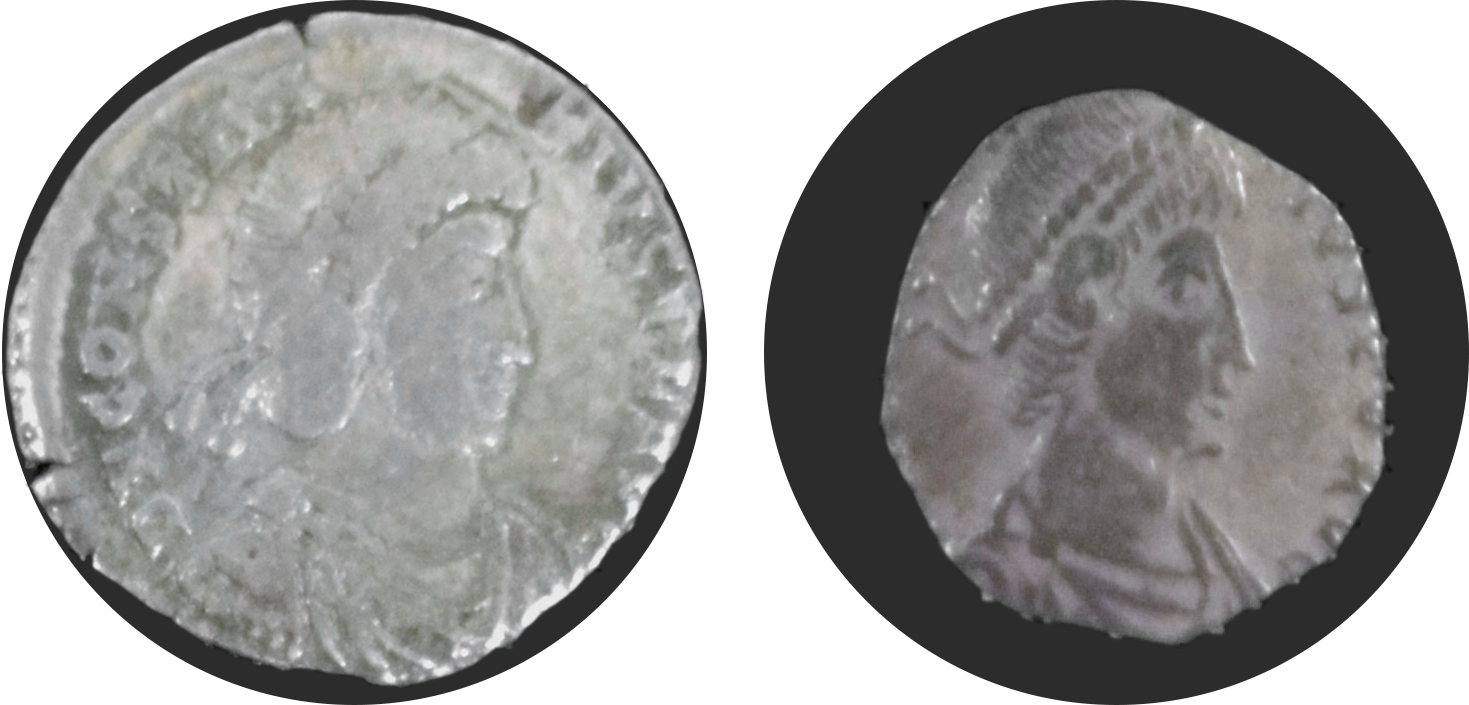
\includegraphics{assets/images/clipped-coins.png}
  \caption{Clipped silver coins of varying severity.}
  \label{fig:clipped-coins}
\end{figure}

Even with these methods of coin debasement\footnote{Besides clipping, sweating
(shaking the coins in a bag and collecting the dust worn off) and plugging
(punching a hole in the middle and hammering the coin flat to close the hole)
were the most prominent methods of coin debasement. \cite{wiki:coin-debasement}}
kept in check, coins still suffer from other issues. They are bulky and not very
convenient to transport, especially when large transfers of value need to
happen. Showing up with a huge bag of silver dollars every time you want to buy
a Mercedes isn't very practical.

Speaking of German things: How the United States \textit{dollar} got its name is
another interesting story. The word \enquote{dollar} is derived from the German word
\textit{Thaler}, short for a \textit{Joachimsthaler}~\cite{wiki:thaler}. A
Joachimsthaler was a coin minted in the town of \textit{Sankt Joachimsthal}.
Thaler is simply a shorthand for someone (or something) coming from the valley,
and because Joachimsthal was \textit{the} valley for silver coin production,
people simply referred to these silver coins as \textit{Thaler.} Thaler (German)
morphed into daalders (Dutch), and finally dollars (English).

\begin{figure}
  \centering
  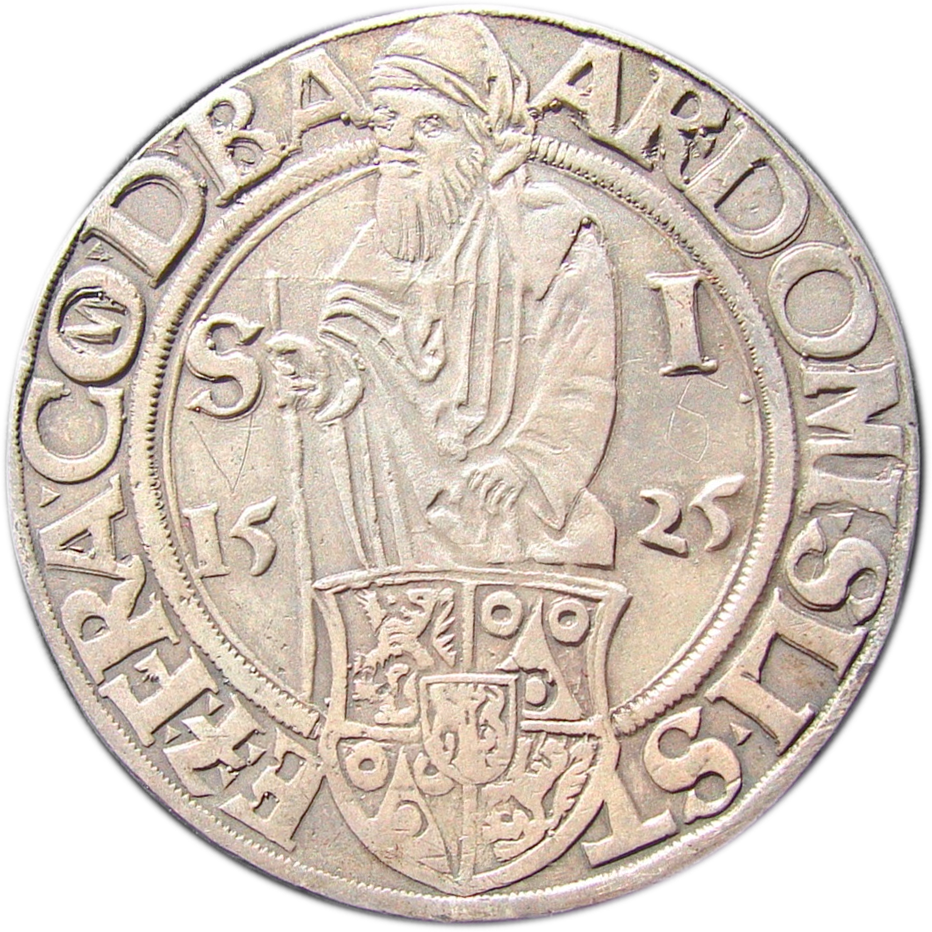
\includegraphics[width=5cm]{assets/images/joachimsthaler.png}
  \caption{The original `dollar'. Saint Joachim is pictured with his robe and wizard hat. Picture cc-by-sa Wikipedia user Berlin-George}
  \label{fig:joachimsthaler}
\end{figure}

The introduction of representative money heralded the downfall of hard
money. Gold certificates were introduced in 1863, and about fifteen
years later, the silver dollar was also slowly but surely being replaced
by a paper proxy: the silver certificate. \cite{wiki:silver-certificate}

It took about 50 years from the introduction of the first silver
certificates until these pieces of paper morphed into something that we
would today recognize as one U.S. dollar.

\begin{figure}
  \centering
  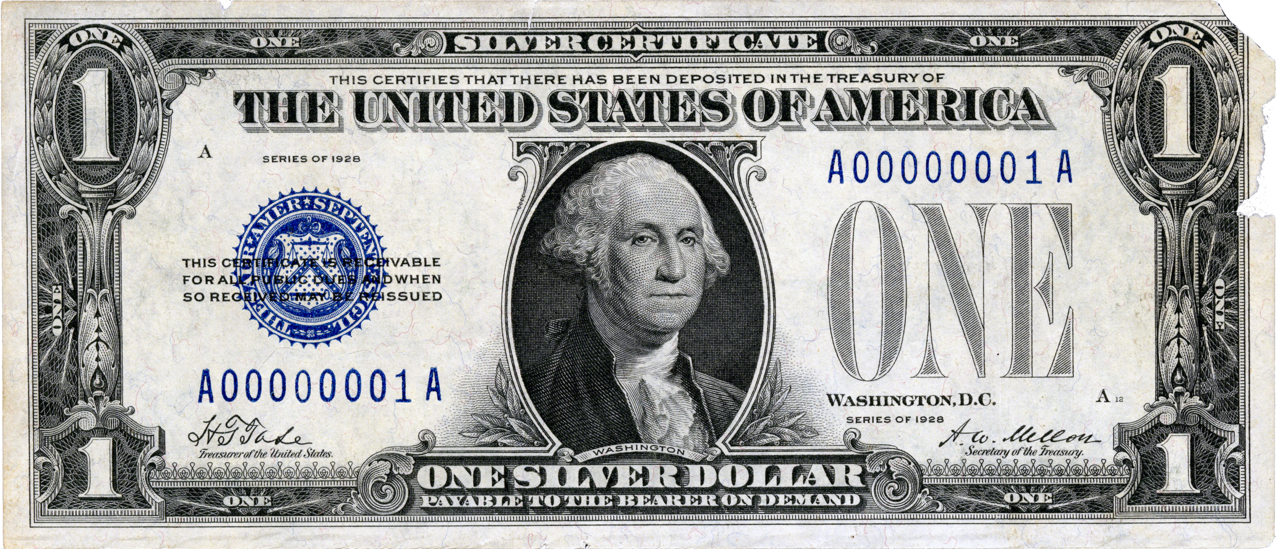
\includegraphics{assets/images/us-silver-dollar-note-smaller.png}
  \caption{A 1928 U.S. silver dollar. `Payable to the bearer on demand.' Picture credit to the National Numismatic Collection at the Smithsonian Institution}
  \label{fig:us-silver-dollar-note-smaller}
\end{figure}

Note that the 1928 U.S. silver dollar above still goes by the name of
\textit{silver certificate}, indicating that this is indeed simply a document
stating that the bearer of this piece of paper is owed a piece of
silver. It is interesting to see that the text which indicates this got
smaller over time. The trace of \enquote{certificate} vanished completely after
a while, being replaced by the reassuring statement that these are
federal reserve notes.

As mentioned above, the same thing happened to gold. Most of the world was on a
bimetallic standard~\cite{wiki:bimetallism}, meaning coins were made
primarily of gold and silver. Having certificates for gold, redeemable in gold
coins, was arguably a technological improvement. Paper is more convenient,
lighter, and since it can be divided arbitrarily by simply printing a smaller
number on it, it is easier to break into smaller units.

To remind the bearers (users) that these certificates were
representative for actual gold and silver, they were colored accordingly
and stated this clearly on the certificate itself. You can fluently read
the writing from top to bottom:

\begin{quotation}
``This certifies that there have been deposited in the treasury of the
United States of America one hundred dollars in gold coin payable to
the bearer on demand.''
\end{quotation}

\begin{figure}
  \centering
  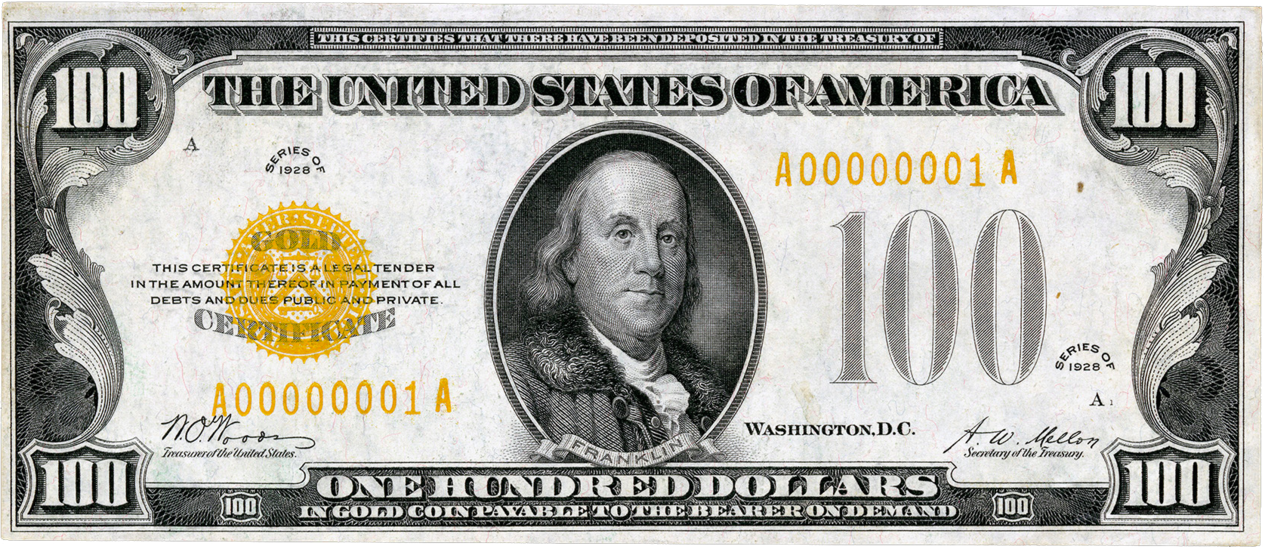
\includegraphics{assets/images/us-gold-cert-100-smaller.png}
  \caption{Picture credit to National Numismatic Collection, National Museum of American History.}
  \label{fig:us-gold-cert-100-smaller}
\end{figure}

In 1963, the words \enquote{PAYABLE TO THE BEARER ON DEMAND} were removed from
all newly issued notes. Five years later, the redemption of paper notes
for gold and silver ended.

The words hinting on the origins and the idea behind paper money were
removed. The golden color disappeared. All that was left was the paper
and with it the ability of the government to print as much of it as it
wishes.

With the abolishment of the gold standard in 1971, this century-long
sleight-of-hand was complete. Money became the illusion we all share to
this day: fiat money. It is worth something because someone commanding
an army and operating jails says it is worth something. As can be
clearly read on every dollar note in circulation today, \enquote{THIS NOTE IS
LEGAL TENDER}. In other words: It is valuable because the note says so.

\begin{figure}
  \centering
  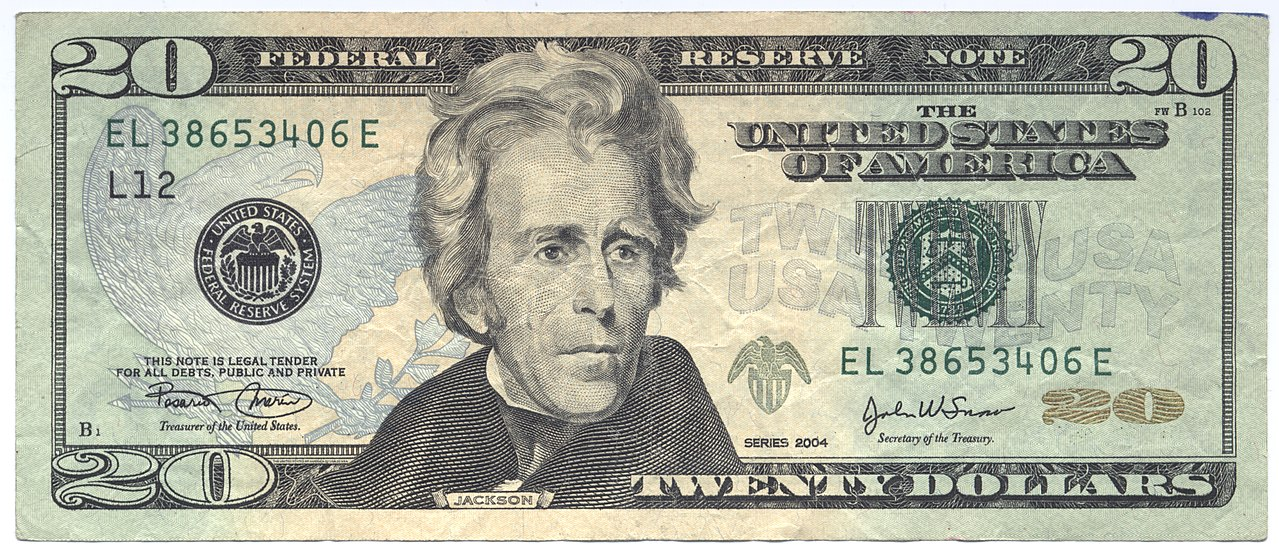
\includegraphics{assets/images/us-dollar-2004.jpg}
  \caption{A 2004 series U.S. twenty dollar note used today. `THIS NOTE IS LEGAL TENDER'}
  \label{fig:us-dollar-2004}
\end{figure}

By the way, there is another interesting lesson on today's bank notes,
hidden in plain sight. The second line reads that this is legal tender
\enquote{FOR ALL DEBTS, PUBLIC AND PRIVATE}. What might be obvious to economists
was surprising to me: All money is debt. My head is still hurting
because of it, and I will leave the exploration of the relation of money
and debt as an exercise to the reader.

As we have seen, gold and silver were used as money for millennia. Over
time, coins made from gold and silver were replaced by paper. Paper
slowly became accepted as payment. This acceptance created an
illusion --- the illusion that the paper itself has value. The final
move was to completely sever the link between the representation and the
actual: abolishing the gold standard and convincing everyone that the
paper in itself is precious.

\paragraph{Bitcoin taught me about the history of money and the greatest sleight of
hand in the history of economics: fiat currency.}

% ---
%
% #### Down the Rabbit Hole
%
% - [Shelling Out: The Origins of Money] by Nick Szabo
% - [Methods of Coin Debasement][coin debasement], [Thaler], [U.S. Silver Certificate][silver certificates], [Bimetallism][bimetallic standard] on Wikipedia
%
% [oldest coin]: https://www.britishmuseum.org/explore/themes/money/the_origins_of_coinage.aspx
% [coin debasement]: https://en.wikipedia.org/wiki/Methods_of_coin_debasement
% [Thaler]: https://en.wikipedia.org/wiki/Thaler
% [Berlin-George]: https://en.wikipedia.org/wiki/File:Bohemia,_Joachimsthaler_1525_Electrotype_Copy._VF._Obverse..jpg
% [silver certificates]: https://en.wikipedia.org/wiki/Silver_certificate_%28United_States%29
% [bimetallic standard]: https://en.wikipedia.org/wiki/Bimetallism
% [Shelling Out: The Origins of Money]: https://nakamotoinstitute.org/shelling-out/
%
% <!-- Wikipedia -->
% [alice]: https://en.wikipedia.org/wiki/Alice%27s_Adventures_in_Wonderland
% [carroll]: https://en.wikipedia.org/wiki/Lewis_Carroll
